\let\negmedspace\undefined
\let\negthickspace\undefined
\documentclass[journal]{IEEEtran}
\usepackage[a5paper, margin=10mm, onecolumn]{geometry}
%\usepackage{lmodern} % Ensure lmodern is loaded for pdflatex
\usepackage{tfrupee} % Include tfrupee package

\setlength{\headheight}{1cm} % Set the height of the header box
\setlength{\headsep}{0mm}     % Set the distance between the header box and the top of the text

\usepackage{gvv-book}
\usepackage{gvv}
\usepackage{cite}
\usepackage{amsmath,amssymb,amsfonts,amsthm,mathtools}
\usepackage{algorithmic}
\usepackage{graphicx}
\usepackage{textcomp}
\usepackage{xcolor}
\usepackage{txfonts}
\usepackage{listings}
\usepackage{enumitem}
\usepackage{mathtools}
\usepackage{gensymb}
\usepackage{comment}
\usepackage[breaklinks=true]{hyperref}
\usepackage{tkz-euclide} 
\usepackage{listings}
\def\inputGnumericTable{}                                 
\usepackage[latin1]{inputenc}                                
\usepackage{color}                                            
\usepackage{array}                                            
\usepackage{longtable}                                       
\usepackage{calc}                                             
\usepackage{multirow}                                         
\usepackage{hhline}                                           
\usepackage{ifthen}                                           
\usepackage{lscape}
\begin{document}

\bibliographystyle{IEEEtran}
\vspace{3cm}

\title{9.2.35}
\author{EE24BTECH11002 - Agamjot Singh}
% \maketitle
% \newpage
% \bigskip
{\let\newpage\relax\maketitle}
%\maketitle

\renewcommand{\thefigure}{\theenumi}
\renewcommand{\thetable}{\theenumi}
\setlength{\intextsep}{10pt} % Space between text and floats

\textbf{Question:}
\newline
Sketch the region $\brak{x, 0} \colon y = \sqrt{4 - x^2}$ and $x$-axis. Find the area of the region using integration.
\newline
\textbf{Solution:}

\begin{table}[h!]
	\centering
	\begin{tabular}[12pt]{ |c| c|}
    \hline
    \textbf{Variable} & \textbf{Description}\\ 
    \hline
	$\vec{A}$ & Point to be found\\
    \hline
	$\vec{B}$ & $(0, 0)$ point\\
    \hline
	$\vec{C}$ & $(6, 0)$ point\\
    \hline
	$\vec{\angle \vec{ABC}}$ & $60 \degree$\\ 
    \hline
    \end{tabular}
	\caption{Variables Used}
	\label{tab9.2.35}
\end{table}

The general equation of a circle is given by 
\begin{align}
	\norm{\vec{x}}^2 + 2\vec{u}^\top\vec{x} + f = 0
\end{align}
The given curve $y = \sqrt{4 - x^2}$ is that of a semicircle, since $y \geq 0$.
\newline
The equation of the curve can be written as
\begin{align}
	x^2 + y^2 - 4 = 0, y \geq 0
\end{align}
The parameters of the circle are
\begin{align}
	\vec{u} = \myvec{0\\0}, f = -4 \implies r = 2, \vec{O} = \myvec{0\\0}
\end{align}
The area between the curve and $x$-axis can be given by
\begin{align}
	A &= \int_{-2}^{2} \sqrt{4 - x^2} \, dx\\
	\text{Substituting } x = 2\sin{\theta} \text{,}\\
	A &= \int_{\frac{-\pi}{2}}^{\frac{\pi}{2}} 4\cos^2{\theta} \, d\theta\\
	A &= 8\int_{0}^{\frac{\pi}{2}} \cos^2{\theta} \, d\theta\\
	A &= 8\int_{0}^{\frac{\pi}{2}} \sin^2{\theta} \, d\theta\\
	\implies 2A &= 8\brak{\frac{\pi}{2}}\\
	\implies A &= 2\pi
\end{align}

\begin{figure}[h!]
   \centering
   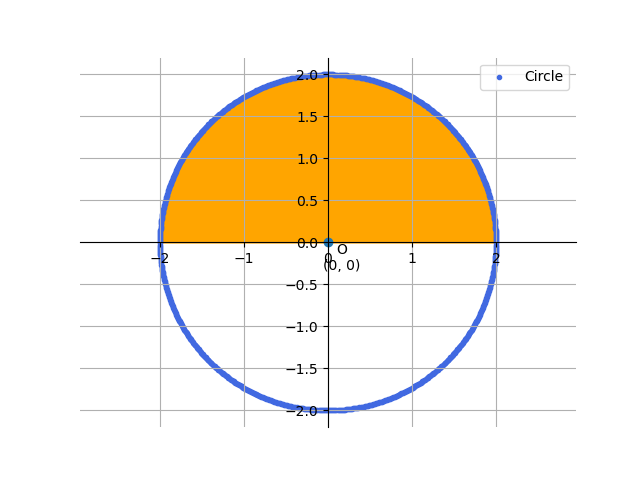
\includegraphics[width=0.7\linewidth]{figs/graph.png}
   \caption{Shaded area representing area of region given}
\end{figure}

\end{document}
